%%%%%%%%%%%%%%%%%%%%%%%%%%%%%%%%%%%%%%%%%%%%%%%%%%%
%%         Arduino and Physical Etoys            %%
%%                                               %%
%%                GIRA 2011                      %%
%% Planète Sciences 20011 for the Latex version) %%
%%%%%%%%%%%%%%%%%%%%%%%%%%%%%%%%%%%%%%%%%%%%%%%%%%%

%% Authors: Ricardo Moran
%% (translation to LaTex: Séverin Lemaignan)


\documentclass[a4paper,12pt]{article}

\usepackage{fullpage}

\usepackage{graphicx}

\usepackage{xcolor}

\usepackage{ifthen}

\usepackage[utf8]{inputenc}

\usepackage[T1]{fontenc}
\pdfmapfile{+ubuntu-regular.map}
\pdfmapfile{+ubuntu-it.map}
\pdfmapfile{+ubuntu-bold.map}
\renewcommand{\rmdefault}{Ubuntu}

\usepackage{listings}
\usepackage{framed}
\usepackage{wrapfig}
\usepackage{fancyhdr} %headers and footers
\pagestyle{fancy}

\usepackage{url}
\usepackage{hyperref}
\usepackage{sectsty}

\usepackage{enumerate}

\usepackage{pdfpages} %% To add a cover to the doc

% Fixme notes
\usepackage[draft,footnote,marginclue]{fixme}

\usepackage[toc]{glossaries}

\usepackage[english]{babel}

%%%%%%%%%%%%%%%%%%%%%%%%%%%%%%%%%%%%%%%%%%%%%%%%%%%%%%%%%%%%%%%%%%%%%%%%%%%%%%%
%%                           Glossary                                        %%
%%%%%%%%%%%%%%%%%%%%%%%%%%%%%%%%%%%%%%%%%%%%%%%%%%%%%%%%%%%%%%%%%%%%%%%%%%%%%%%
\makeglossaries

\newglossaryentry{halo}
		{name={halo}, 
		description={}
		}
%%%%%%%%%%%%%%%%%%%%%%%%%%%%%%%%%%%%%%%%%%%%%%%%%%%%%%%%%%%%%%%%%%%%%%%%%%%%%%%

\def\appName{Physical Etoys}

\def\rc{right clic~}
\def\mc{middle clic~}
\def\lc{left clic~}


\newcommand{\screenshot}[1]
{
\begin{center}
	\includegraphics[scale=0.5]{images/#1}
\end{center}
}

\newcommand{\tile}[1]{
\sffamily
\fcolorbox[RGB]{200,192,144}{200,248,200}{\textbf{#1}}
\normalfont
}

\newcommand{\testtile}[1]
{
\sffamily
\fcolorbox[RGB]{255,239,198}{247,222,189}{
\ifthenelse {\equal{#1} {}} {\textbf{Test: Yes/No}} {\textbf{#1}}
}
\normalfont
}

% Useful for code or script names
\newcommand{\code}[1]{\texttt{#1}}

\newcommand{\important}[1]{\textbf{#1}}

\newcommand{\keyword}[2]{\important{\gls{#1}}}


\newcommand{\inserticon}[1]
{
\includegraphics[scale=0.5]{../shared/images/icons/#1.png}
}
% Use this macro to easily insert halo icons in the doc.
% \icon{icon_name} insert inline the icon ;
% \icon[name]{icon_name} display "the [image] <name> icon"
%
% Available icons are:
% clone, close, exclamation, eye, grab, greenarrow, menu, minimize, myselftile,
% pausescript, redraw, rotate, scale, script, startscript, toolbox, variable
\newcommand{\icon}[2][]
{
\ifthenelse {\equal{#1} {}} {\inserticon{#2}} {the \inserticon{#2} \important{#1} icon}
}

% Used for section that must be done by the reader
\newcommand{\todo}[1]
{
#1
}

\newcommand{\tip}[1]
{
\begin{framed}
%\marginpar{#1}
%[RGB]{214,141,0}{251,240,220}
\begin{wrapfigure}[3]{l}{1.8em}
	\vspace{-15pt}
	
\includegraphics[width=2.0em]{../shared/images/tip.png}
\end{wrapfigure}
#1
\end{framed}
}


% Set default font to scriptsize and sans-serif for margin notes
\let\myMargin\marginpar
\renewcommand{\marginpar}[1]{\myMargin{{\scriptsize \sffamily #1}}}


%################# Header and footer with fancyhdr
\headheight=14.85pt
% Section section name in lower case
%\renewcommand{\chaptermark}[1]{\markboth{#1}{}} %only when doc type = book
%\renewcommand{\sectionmark}[1]{\markright{#1}}

\fancyhf{}
\fancyhead[RO,LE]{\scriptsize\bfseries\leftmark}
%\fancyhead[LE]{\rightmark}
\fancyfoot[LE,RO]{\bfseries\thepage}
\renewcommand{\headrulewidth}{0.3pt}
%\addtolength{\headheight}{2pt}
\addtolength{\headsep}{20pt}
\addtolength{\footskip}{10pt}
\renewcommand{\footrulewidth}{0pt}
\fancypagestyle{plain}{\fancyhead{}\renewcommand{\headrulewidth}{0pt}}

%%%%%%%%%%%%%%%%%%%%%%%%%%%%%%%%%%%%%%%%%%%%%%%%%%%%%%%%%%%%%%%%%%%%%%%%%%%%%%%%%
%%%%%%%%%%%%%%%%%%%%%%%%%%%%%%%%%%%%%%%%%%%%%%%%%%%%%%%%%%%%%%%%%%%%%%%%%%%%%%%%%

\title{
	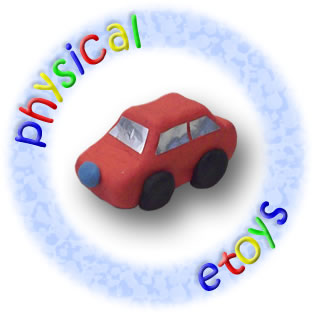
\includegraphics[width=8cm]{../shared/images/physical_etoys_logo.jpg}\\
	\vfill
	%
\includegraphics[width=5cm]{minibot.png}
	\vspace{3em}
	\LARGE{\textbf{\appName~and the Arduino board}}\\[1cm]
	\large{Step by step into Arduino programming with \appName}\\[1cm]
	\vfill
}

\author{
GIRA
}

%%%%%%%%%%%%%%%%%%%%%%%%%%%%%%%%%%%%%%%%%%%%%%%%%%%%%%%%%%%%%%%%%%%%%%%%%%%%%%%%%
%%%%%%%%%%%%%%%%%%%%%%%%%%%%%%%%%%%%%%%%%%%%%%%%%%%%%%%%%%%%%%%%%%%%%%%%%%%%%%%%%
\begin{document}

% If a PDF file called 'cover.pdf' exists, use it as cover.
\IfFileExists{cover.pdf}{
\includepdf[pages=-, fitpaper]{cover.pdf}
\thispagestyle{empty}
\cleardoublepage
}

\maketitle

\cleardoublepage
\tableofcontents
\cleardoublepage

Due to the popularity and the different features that the Arduino board has, in
this tutorial we will see how to access to some of them from Physical Etoys in
order to make simple programs and have a suitable introduction to electronics.  

%%%%%%%%%%%%%%%%%%%%%%%%%%%%%%%%%%%%%%%%%%%%%%%%%%%%%%%%%%%%%%%%%%%%%%%%%%%%%%%%%
\section{Installation}

\subsection{Necessary tools}

\begin{itemize}
	\item An Arduino board (we have worked with a Duemilanove).
	\item An USB cable.
	\item Physical Etoys software.
\end{itemize}

\subsection{Optional tools}

A LED, a pushbutton, a protoboard, 3 10 KOhms resistors and a servomotor (to
prove that the board works). 

\subsection{Driver installation}

When you connect the board, Windows should initiate the driver installation
process (if you haven't used the computer with an Arduino board before).

On Windows Vista, the driver should be automatically downloaded and installed.

On Windows XP, the Add New Hardware wizard will open:

\begin{itemize}
	
	\item When asked: Can Windows connect to Windows Update to search for
	software? Select No, not this time. Click next.

	\item Select Install from a list or specified location (Advanced) and click
	next.

	\item Make sure that Search for the best driver in these locations is
	checked; uncheck Search removable media; check “Include this location in
	the search” and browse the drivers in the /FTDI USB Drivers directory of
	the Arduino distribution. (The latest version of the drivers can be found
	on the FTDI website). Click next.

	\item The wizard will search for the driver and then tell you that a "USB
	Serial Converter" was found. Click finish.

	\item The new hardware wizard will appear again. Go through the same steps
	and select the same options and location to search. This time, a "USB
	Serial Port" will be found.

\end{itemize}

You can check that the drivers have been installed by opening the Windows
Device Manager (in the Hardware tab of System control panel). Look for a "USB
Serial Port" in the Ports section; that's the Arduino board.


%%%%%%%%%%%%%%%%%%%%%%%%%%%%%%%%%%%%%%%%%%%%%%%%%%%%%%%%%%%%%%%%%%%%%%%%%%%%%%%%%
\section{Connecting Arduino to Physical Etoys}

First and foremost, inside Physical Etoys, we have to get an “Arduino board”.
This is a graphical object that represents the Arduino board. 

In order to obtain it we have to open the supplies’ flap.

\screenshot{01.png}

The supplies’ flap contains the most used objects.  As long as we use the
system we are going to learn more things about them. The one that interests us
is the “Object catalog”.

\screenshot{02.png}

Now we have to drop the object catalog on the world. 

\screenshot{03.png}

The object catalog is like a box that contains the entire objects that we can
use. It is ordered by categories but we can arrange the objects alphabetically.
Apart from that we can look for a particular one.

Now we have to choose the Electronics category. Then we have to drag the
“Arduino board” etoy and place it on the world.

\screenshot{04.png}
  
Now we have to open its viewer by making right-click on the “Arduino board” to
open the halo. The halo is a set of buttons which surround the object and let
the user modify, move, delete and maximize it.  

Next we click on the viewer icon (light blue) to make it appear. The viewer is
a flap where we can not only see and modify the object’s properties on the
screen but also create scripts for them to perform actions like moving on the
screen. The properties and the actions are represented as tiles.

\screenshot{05.png}


In a special category called “arduino-connection” we can find instructions
which are useful for connecting with the Arduino board. In order to change
categories we have to double click the tiny triangle which is on the left hand
side of the title of the categories and then we have to choose the desired
category. 

\screenshot{06.png}

First we have to specify which board we are going to use.  In this case we will
choose the Duemilanove board with the ATmega328 microcontroller. Then we have
to define the COM port the board is connected. To know where is connected, we
have to right-click in My computer$\rightarrow$properties. Next, inside the
hardware tab we have to click on the device manager. 

\screenshot{07.png}

Now we have to look for the “ports” section and once inside, the port number
will be next to the label “USB Serial Port”. In this case the port is 8. 
 
\screenshot{08.png}

Therefore, the value of the tile which corresponds to the port will be COM 8

\screenshot{09.png}


Now the important instruction is “connect”. If we run this instruction (by
clicking on \icon[exclamation]{exclamation}) we will connect the Arduino with
Physical Etoys and then the tile which indicates if the Arduino board is
connected will change its value to \code{true}. 

\screenshot{10.png}

If this is the first time that we have tried to connect the Arduino board, a
pop up will appear asking if you want to install Firmata. Firmata is a program
which contains the communication protocol to enable the board to receive
orders. So, we click on the yes button. 

\screenshot{11.png}


A bar will show the installation progress.
 
\screenshot{12.png}

If no error occurred, a caption will appear indicating that the process ended
correctly. Now we have to connect the Arduino board again (by clicking on the
exclamation sign of the connect tile). If the Arduino board is connected, the
value of the isConnected tile will become true. 

\screenshot{13.png}

%%%%%%%%%%%%%%%%%%%%%%%%%%%%%%%%%%%%%%%%%%%%%%%%%%%%%%%%%%%%%%%%%%%%%%%%%%%%%%%%%
\section{The “hello world” of electronics (blinking a led)}

Before working with Physical Etoys we need to connect physically the led with
the board. In this example, the cathode must be connected to ground and the
anode to the thirteenth pin. 

\screenshot{14.jpg}

\screenshot{15.png}

Now we can start with Physical Etoys. 

Inside the “electronics category” from the object catalog, we drag a led. 

\screenshot{16.png}

Once dropped, we have click on the positive pin and drag the appearing cable to
one of the digital pins of the “Arduino board” (in this case the thirteen pin). 

\screenshot{17.png}

Next we go to the led’s viewer and these tiles will appear:

\screenshot{18.png}

Now we have to create a new script to make the led blinks. To create a new
script we have to drag the \tile{empty script} tile which is inside the
“scripts” category.  Once dragged we will see this:

\screenshot{19.png}

Then we have to click on \icon[toolbox]{toolbox} and choose a \testtile{} tile.
This tile means that the script will do something according to a condition (in
this case the led’s value). For the ones who have a bit of experience in
programming this tile is an “if structure”. 

\screenshot{20.png}

In order to establish the condition, we will drag (not from the arrow because
we do not want to assign values to variables) the “led value tile” next to
“test”:

\screenshot{21.png}

Now we have to define what the script will do if the led is turned on.
Obviously, it has to turn it off. So we will assign to “led value” a false
value. So we have to drag the led value from the arrow because we want to
assign a value to the variable. 


\screenshot{22.png}

\screenshot{22b.png}


Now we will do the same but with a subtle difference: when the led is off,
Physical Etoys will turn it on.  So we have to drag from the \icon{greenarrow}
arrow the \tile{led value} tile to the \testtile{No} section of the \testtile{}
tile but we will change its value to true. 

\screenshot{23.png}

Finally we will run the script by clicking on \icon[clock]{startscript}. 

\screenshot{24.png}

If everything was fine, the led will blink.

%%%%%%%%%%%%%%%%%%%%%%%%%%%%%%%%%%%%%%%%%%%%%%%%%%%%%%%%%%%%%%%%%%%%%%%%%%%%%%%%%
\section{Turning on a led by pressing a button}

Inside the Electronics category we have to drag a “push button” and then we
have to connect it to the second pin of the “Arduino board”.

\screenshot{25.png}

Take into account not to disconnect the led from the thirteen pin. Apart from
that, stop the led’s script because it will interfere with the objective of
this exercise.

The physical connection of the button (with the resistor and the protoboard)
should be like this:

\screenshot{26.png}

\screenshot{27.png}

Now we have to enter to the Pushbutton’s viewer and create a new script. 

\screenshot{28.png}

Then we add a \testtile{} tile to know when the button is pressed. We have to
drag the tile from its name because it is not an assignment. We want to consult
its value. 

\screenshot{29.png}

In case the button is pressed we will assign to the led a \code{true} value,
otherwise we will assign a false value. Remember to drag the tiles from the
\icon{greenarrow} arrows. Finally we have to click on \icon[clock]{startscript}
to run the script. 

\screenshot{30.png}

If everything was fine, when we press the button, the led will blink. 

%%%%%%%%%%%%%%%%%%%%%%%%%%%%%%%%%%%%%%%%%%%%%%%%%%%%%%%%%%%%%%%%%%%%%%%%%%%%%%%%%
\section{Reading a Photoresistor}

As we have the “Arduino Board” connected, we will attach a Photoresistor (which
is inside the electronics category) to the second analog input pin.

\screenshot{31.png}

The real connection should be more or less like this:

\screenshot{32.png}

\screenshot{33.png}

Next we open the photoresistor’s viewer and create a new script. Now we have to
go to the object catalog and drag from the basic category a rectangle. Then we
open the rectangle’s viewer in order to drag (from the arrow) the brightness
tile inside the photoresistor’s script. Now we have to open the photoresistor’s
viewer to replace the rectangle’s brightness value (\tile{100}) with the
\tile{Photoresistor’s light value} tile (not from the arrow because we only
want to read the value). 

\screenshot{34.png}

Finally we run the script to see how the rectangle changes its brightness
according to the ambient light. 

%%%%%%%%%%%%%%%%%%%%%%%%%%%%%%%%%%%%%%%%%%%%%%%%%%%%%%%%%%%%%%%%%%%%%%%%%%%%%%%%%
\section{Rotate a Servo with a rectangle}

As we have the “Arduino Board” connected, we will attach a Servo (which is
inside the electronics category) to the seventh pin. 

\screenshot{35.png}

The physical connection should be like this: 

\screenshot{36.png}

In order to save time we can use the rectangle created in the last exercise. We
open its halo and then we drag \icon[scale]{scale} to change its size. 

\screenshot{37.png}

Now we have to open the servo’s viewer and create a new script with the tile
that contains the servo’s degrees. Remember that it is an assignment;
therefore, we will drag the tile from the \icon{greenarrow} arrow. 

\screenshot{38.png}

Then we have to open the rectangle’s viewer and inside the basic category we
have to drag (from its value) the \tile{heading} tile. Next we run the script. 

\screenshot{39.png}

While the script is running we have to open the rectangle’s halo. Finally we
have to drag \icon[rotate]{rotate} to rotate the rectangle. 

\screenshot{40.png}

If everything was fine the motor will move according to the rectangle’s
heading. 

%%%%%%%%%%%%%%%%%%%%%%%%%%%%%%%%%%%%%%%%%%%%%%%%%%%%%%%%%%%%%%%%%%%%%%%%%%%%%%%%%
\section{Conclusion}

Well, that is basically all that we need to begin using the Arduino board. The
possibilities of interaction between the computer, Arduino and the other
electronic components that Physical Etoys provides are very numerous to deal
with everyone in this small tutorial. We encourage you to discover the other
ones by exploring the environment (testing, playing, touching and breaking if
it is necessary) 

Have fun!

%%%%%%%%%%%%%%%%%%%%%%%%%%%%%%%%%%%%%%%%%%%%%%%%%%%%%%%%%%%%%%%%%%%%%%%%%%%%%%%%%
%%%%%%%%%%%%%%%%%%%%%%%%%%%%%%%%%%%%%%%%%%%%%%%%%%%%%%%%%%%%%%%%%%%%%%%%%%%%%%%%%
\printglossaries

%%%%%%%%%%%%%%%%%%%%%%%%%%%%%%%%%%%%%%%%%%%%%%%%%%%%%%%%%%%%%%%%%%%%%%%%%%%%%%%%%%%%%%%%%%%%%%%%%%%%%%%
\clearpage
\thispagestyle{empty}
~
\vfill
\begin{center}
	GIRA 2011\\
	This documentation is provided under the Creative Commons BY-SA license.\\
	\vspace{2cm}
	
\includegraphics[scale=0.5]{../shared/images/logo_cc.png}
\end{center}

\vfill

\begin{center}
	The original LaTeX sources of this document can be downloaded from GitHub.
	\url{http://github.com/GIRA/Physical-Etoys}
\end{center}

\vfill

\end{document}

